\newpage
\subsection{Graphisches Ableiten Beispiele}

\hfill \break
\begin{itemize}
    \item \textcolor{blue}{Funktion}
    \item \textcolor{red}{Ableitung}
\end{itemize}

\hfill \break
Example $f(x) = 2x-1$:\\
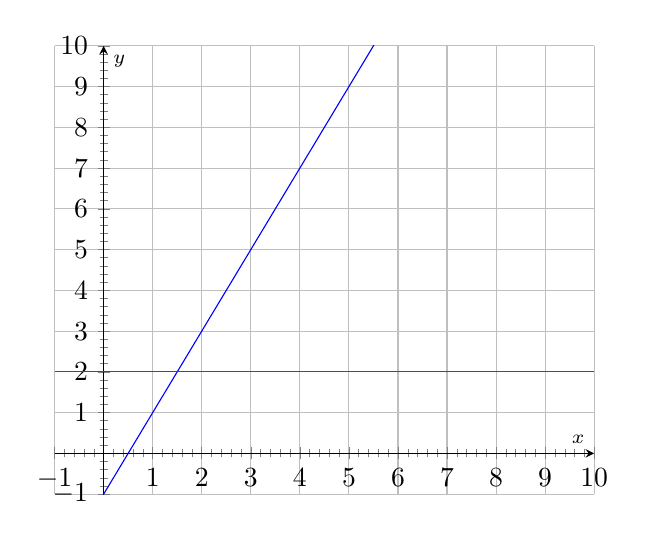
\begin{tikzpicture}[scale=1]
    \begin{axis}%
        [
            grid=major,
            xtick={-1,0,...,10},
            minor x tick num=4,
            xmin=-1,
            xmax=10,
            xlabel={\scriptsize $x$},
            axis x line=middle,
            ytick={-1,0,...,10},
            minor y tick num=4,
            ymin=-1,
            ymax=10,
            ylabel={\scriptsize $y$},
            axis y line=middle,
            no markers,
            samples=100,
            domain=-1:10,
        ]
        \addplot[blue] (x,{2*x-1});
        \addplot[red] (x,{2});
    \end{axis}
\end{tikzpicture}

\hfill \break
Example $f(x) = ((x-1)^2)-1$:\\
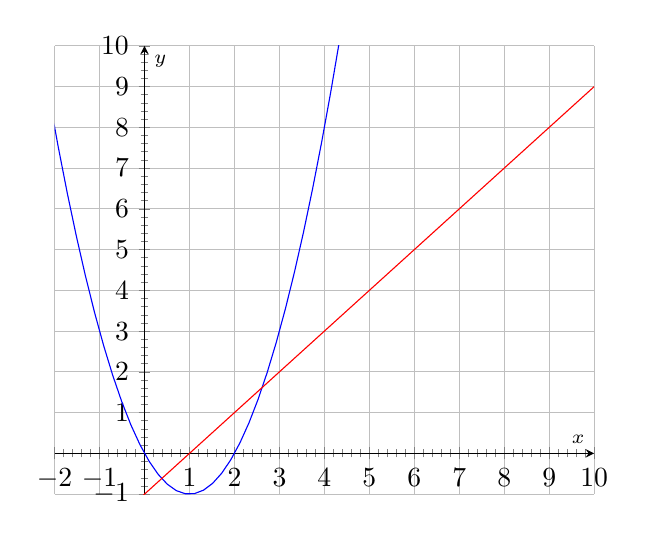
\begin{tikzpicture}[scale=1]
    \begin{axis}%
        [
            grid=major,
            xtick={-2,-1,...,10},
            minor x tick num=4,
            xmin=-2,
            xmax=10,
            xlabel={\scriptsize $x$},
            axis x line=middle,
            ytick={-1,0,...,10},
            minor y tick num=4,
            ymin=-1,
            ymax=10,
            ylabel={\scriptsize $y$},
            axis y line=middle,
            no markers,
            samples=100,
            domain=-10:10,
        ]
        \addplot[blue] (x,{((x-1)^2)-1});
        \addplot[red] (x,{2(x-1)});
    \end{axis}
\end{tikzpicture}